\subsection{Batterij} \label{sec:battery}
In onderzoek \cite{BatteryComparison} is te zien dat Lithium-Polymeer batterijen (LiPo) een hoge energiedichtheid hebben in vergelijking met andere soorten batterijen. Er zijn anderen die hogere energie densiteit hebben, maar daarvan zijn de kosten hoog, of zijn er andere nadelige effecten\cite{BatteryComparison}. Dit heeft ervoor gezorgd dat voor de sensor module ontwerp een LiPo gekozen is als batterij. Spanning van een cel LiPo (1s) is maximaal 4.2 V en minimaal veilige spanning is 2.7 V\cite{BatteryComparison}.

\subsection{Voeding} \label{sec:voeding} 

%!! TODO: energy harvesting, spanning, batterij laden, beveiliging, stroom. 

De voedingsspanning is gekozen vanuit de maximale spanning die nodig is voor de ISFET sensor\cite{isfet}. Hieruit volgt een maximale systeemspanning van 3.3 V. 


Zoals te lezen in \cref{sec:battery} is er gekozen voor LiPo batterij technologie. De batterij heeft een beveiliging voor beide op- en ontladen nodig. De celspanning moet omgezet worden naar systeemspanning van 3.3 V. Dit wordt op 2 manieren gedaan, met een DC-DC buck-boost converter en een low dropout regelaar(LDO). De buck-boost is efficiënter dan de LDO. Een voordeel van de LDO is dat de spanningsrimpel veel lager is dan bij een buck-boost. Daarom wordt de LDO gebruikt voor het voeden van de analoge uitleesschakeling. De buck-boost gaat naar het digitale deel. Als een microcontroller goed ontkoppeld is dan maakt het spanningsrimpel niet uit voor de werking van de microcontroller. Daardoor is de hogere rimpel spanning van de buck-boost niet een probleem voor de microcontroller. De voeding is schematisch te zien in \cref{fig:voedingSchematisch}.

Voor energy harvesting is er een piezo element gekozen. Een piezo element kan gezien worden als een AC bron. Deze AC bron moet omgezet worden naar DC die door het systeem gebruikt kan worden om de batterij mee op te laden. De AC bron wordt met een gelijkrichter naar DC omgezet. Deze DC spanning is niet hetzelfde als de systeemspanning dus die moet omgezet worden naar een spanning die de batterij in gaat, zodat de batterij kan opladen.

\begin{figure}[ht]
    \centering 
    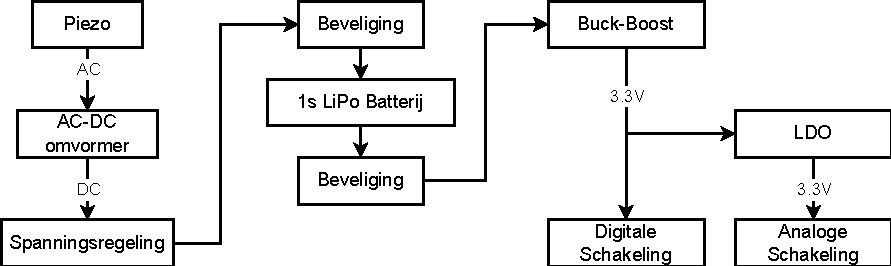
\includegraphics{voedingSchematisch.pdf}
    \caption{Voeding schematisch}
    \label{fig:voedingSchematisch}
\end{figure}





\subsection{Energie budget}
